\documentclass[aspectratio=169,10pt]{beamer}
\usepackage{fontspec}
\usepackage{polyglossia}
\setdefaultlanguage{russian}
\setotherlanguage{english}
\setmainfont{DejaVu Sans}
\usepackage{graphicx}
\setsansfont{DejaVu Sans}
\setmonofont{DejaVu Sans Mono}
\definecolor{teal}{HTML}{0A685B}
\definecolor{dark}{HTML}{153B35}
\definecolor{pale}{HTML}{E8F4EE}
\definecolor{orange}{HTML}{A95A33}
\setbeamercolor{frametitle}{fg=dark}
\setbeamercolor{title}{fg=dark}
\setbeamercolor{structure}{fg=teal}
\setbeamercolor{block title}{bg=teal,fg=white}
\setbeamercolor{block body}{bg=pale,fg=dark}
\setbeamercolor{block title alerted}{bg=orange,fg=white}
\setbeamercolor{block body alerted}{bg=orange!9,fg=dark}
\setbeamertemplate{navigation symbols}{}
\setbeamertemplate{footline}{\hfill\scriptsize\insertframenumber\, / \,\inserttotalframenumber\hspace{12pt}\vspace{5pt}}
\setbeamertemplate{itemize item}{\raisebox{.2ex}{\tiny$\blacktriangleright$}}
\setbeamerfont{frametitle}{size=\Large,series=\bfseries}
\setbeamerfont{normal text}{size=\normalsize}
\setlength{\leftmargini}{1.3em}
\begin{document}
\begin{frame}[plain]
\begin{beamercolorbox}[wd=\paperwidth,ht=\paperheight,sep=1.4cm,center]{title}
\vspace*{1.0cm}{\large Данные как основа ИИ · семестр 2}\par\vspace{1cm}
{\fontsize{30}{38}\selectfont\bfseries Одинаковое среднее —\ разные истории}\par\vspace{0.6cm}
{\large Распределения, выбросы и оценка данных}\par\vfill{\small Кейс «Умный кампус» · университетские пространства}
\end{beamercolorbox}\end{frame}
\begin{frame}[t]{Что на самом деле описывает среднее?}
\vspace{.15cm}\begin{itemize}
\item Две аудитории. Сорок сессий на каждую.\vspace{6pt}
\item Одинаковое среднее CO₂ — 1000 ppm.\vspace{6pt}
\item Можно ли сказать, что условия одинаковы?\vspace{6pt}
\end{itemize}
\vfill\begin{alertblock}{Вопрос аудитории}\large какую информацию мы ещё не знаем?\end{alertblock}
\end{frame}
\begin{frame}[t]{Проверяем данные до статистики}
\vspace{.15cm}\begin{itemize}
\item Единица наблюдения — учебная сессия.\vspace{6pt}
\item Обратите внимание на пропуски, флаги качества и единицы.\vspace{6pt}
\item Отдельно задаём вопрос анализа: типичное состояние или редкие эпизоды?\vspace{6pt}
\end{itemize}
\end{frame}
\begin{frame}[t]{Центр: среднее, медиана, мода}
\vspace{.15cm}\begin{itemize}
\item Среднее использует каждое числовое значение.\vspace{6pt}
\item Медиана делит упорядоченные данные пополам.\vspace{6pt}
\item Мода — наиболее частое значение; зависит от округления.\vspace{6pt}
\end{itemize}
\vfill\begin{alertblock}{Вопрос аудитории}\large какая характеристика устойчивее к редкому пику?\end{alertblock}
\end{frame}
\begin{frame}[t]{Две серии, одно среднее}
\vspace{.15cm}\begin{itemize}
\item A: почти все значения рядом с 1000 ppm.\vspace{6pt}
\item B: чаще ниже 1000 ppm, но бывают редкие пики.\vspace{6pt}
\item Одинаковое среднее не означает одинаковую форму распределения.\vspace{6pt}
\end{itemize}
\end{frame}
\begin{frame}[t]{Гистограмма возвращает детали}
\vspace{.15cm}\begin{itemize}
\item Каждый столбец показывает частоту в интервале.\vspace{6pt}
\item Ширина интервалов влияет на рисунок.\vspace{6pt}
\item Сравнивая группы, используем общие границы и шкалы.\vspace{6pt}
\end{itemize}
\end{frame}
\begin{frame}[t]{Что видно на данных?}
\vspace{.4cm}
\centering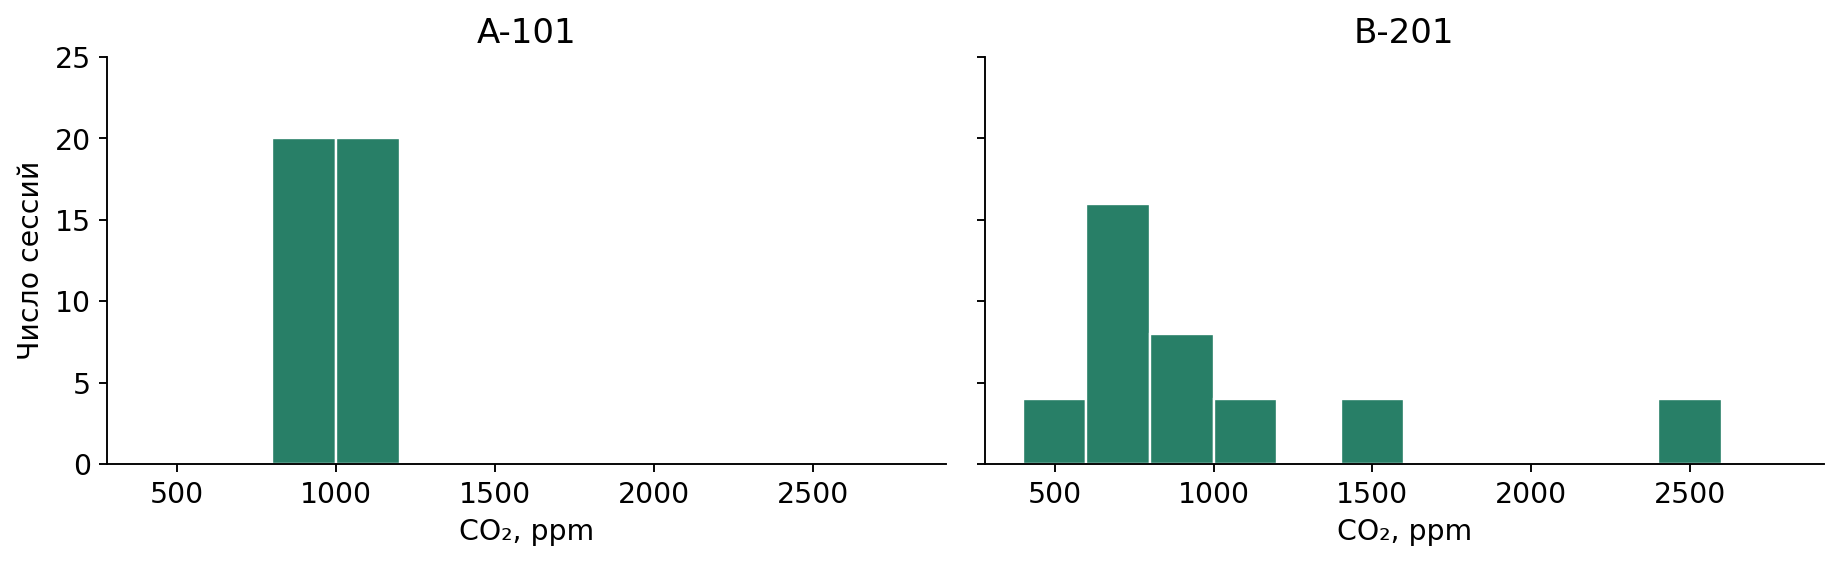
\includegraphics[width=.94\linewidth]{../assets/chart06_distributions.png}
\end{frame}
\begin{frame}[t]{Что скрывает таблица средних?}
\vspace{.15cm}\begin{itemize}
\item A-101: среднее 1000, медиана 1000 ppm.\vspace{6pt}
\item B-201: среднее 1000, медиана 800 ppm.\vspace{6pt}
\item Редкие высокие показания требуют отдельного внимания.\vspace{6pt}
\end{itemize}
\vfill\begin{alertblock}{Вопрос аудитории}\large Какой отчёт точнее отвечает на вопрос управляющего?\end{alertblock}
\end{frame}
\begin{frame}[t]{Разброс: что измерять}
\vspace{.15cm}\begin{itemize}
\item Диапазон и размах чувствительны к крайним значениям.\vspace{6pt}
\item Q1 и Q3 ограничивают центральную половину наблюдений.\vspace{6pt}
\item IQR = Q3 − Q1; стандартное отклонение показывает масштаб разброса.\vspace{6pt}
\end{itemize}
\end{frame}
\begin{frame}[t]{Boxplot — не детектор ошибок}
\vspace{.15cm}\begin{itemize}
\item «Усы» и отдельные точки отмечают статистическую структуру.\vspace{6pt}
\item Отдельная точка не доказывает неисправность прибора.\vspace{6pt}
\item Причина пика требует сопоставления с первичными данными.\vspace{6pt}
\end{itemize}
\vfill\begin{alertblock}{Вопрос аудитории}\large Что запросить у службы эксплуатации?\end{alertblock}
\end{frame}
\begin{frame}[t]{Пик в данных и пик в выводе}
\vspace{.15cm}\begin{itemize}
\item Четыре сессии B-201 по 2500 ppm.\vspace{6pt}
\item Если исключить их из расчёта, среднее уменьшится.\vspace{6pt}
\item Но не было доказано, что эти записи ошибочны.\vspace{6pt}
\end{itemize}
\end{frame}
\begin{frame}[t]{Пропуски меняют состав}
\vspace{.15cm}\begin{itemize}
\item План: по 12 измерений в каждом корпусе.\vspace{6pt}
\item Известно: 11 против 4.\vspace{6pt}
\item Равные группы превращаются в неравные без какой-либо математической ошибки.\vspace{6pt}
\end{itemize}
\end{frame}
\begin{frame}[t]{Как отвечать на вопрос группы}
\vspace{.15cm}\begin{itemize}
\item Сначала обозначьте количество наблюдений.\vspace{6pt}
\item Затем покажите центр, разброс и форму.\vspace{6pt}
\item Наконец, укажите пропуски и условия применимости.\vspace{6pt}
\end{itemize}
\end{frame}
\begin{frame}[t]{ИИ сообщает: «Среднее совпало — всё одинаково»}
\vspace{.15cm}\begin{itemize}
\item Верный расчёт не гарантирует корректную интерпретацию.\vspace{6pt}
\item Проверьте исходные строки, единицы и пропуски.\vspace{6pt}
\item Замените категорический вывод на проверяемое наблюдение.\vspace{6pt}
\end{itemize}
\end{frame}
\begin{frame}[t]{Лабораторная и три маршрута}
\vspace{.15cm}\begin{itemize}
\item Таблицы: паспорт групп и две версии управленческой записки.\vspace{6pt}
\item Python: воспроизводимые расчёты, графики и проверки.\vspace{6pt}
\item Исследование: устойчивость статистик и ограничения данных.\vspace{6pt}
\end{itemize}
\end{frame}
\begin{frame}[t]{Выходной билет}
\vspace{.15cm}\begin{itemize}
\item Когда медиана информативнее среднего?\vspace{6pt}
\item Почему удаление пиков может ухудшить отчёт?\vspace{6pt}
\item Что надо сообщить о пропусках в группах?\vspace{6pt}
\end{itemize}
\end{frame}
\end{document}